\documentclass[tikz,border=5pt]{standalone}
\usetikzlibrary{arrows.meta}
\usetikzlibrary{backgrounds}

\begin{document}
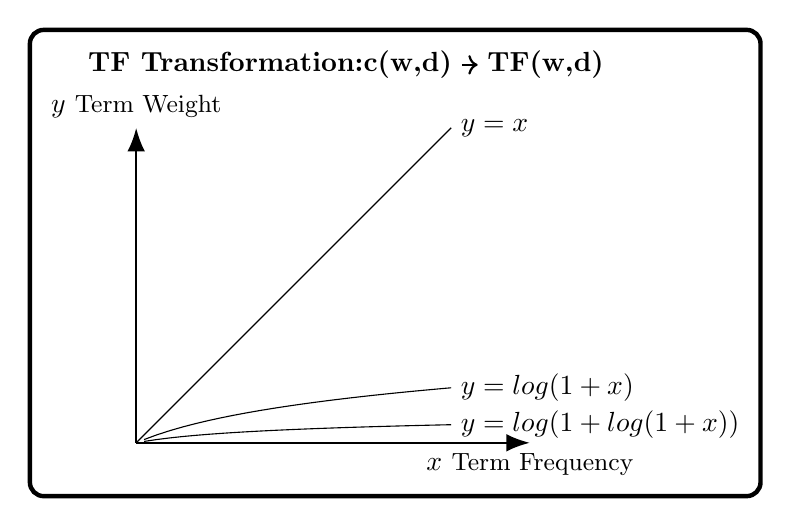
\begin{tikzpicture}
	[framed,background rectangle/.style={ultra thick, rounded corners=5pt, draw}];
	%[framed,background rectangle/.style={double,ultra thick,draw=red, top color=blue, rounded corners}]
	%Axis
	\draw[-{Latex[length=3mm]}, thick] (0,0)--(5,0) node[below]{$x$ \small Term Frequency};
	\draw[-{Latex[length=3mm]}, thick] (0,0)--(0,4) node[above]{$y$ \small Term Weight};

	%coordinate
	%\draw (0,0) -- (45:5) node[anchor=west]{$\small y=x$};
	%\draw plot [domain=0.1:4] (\x,{log2(\x)});
	%\draw[color=blue,domain=0.067:4.5,samples=100] plot (\x,{(0.3)/(\x)});
	%\clip (0,0) rectangle (5,3);
	\draw plot [domain=0:4] (\x,\x) node[anchor=west]{$\small y=x$};
	\draw plot [domain=0.1:4] (\x,{log10(1+\x)}) node[anchor=west]{$\small y=log(1+x)$} ;
	\draw plot [domain=0.1:4] (\x,{log10(1+log10(1+\x))}) node[anchor=west]{$\small y=log(1+log(1+x))$};
	

	%title
	%font =\fontsize{20pt}{0}\selectfont
	%\node[above, font=\bfseries] at (current bounding box.north) {TF Transformation: c(w,d) TF(w,d)};
	\node (titleA) [font=\bfseries] at (1.7,4.8) {TF Transformation:c(w,d)};
	\node (titleB) [font=\bfseries] at (5.2,4.8) {TF(w,d)};
	\draw[->,thick] (titleA) -- (titleB);
\end{tikzpicture}
\end{document}